% Definition der Klasse des Dokumentes
\documentclass[11pt, a4paper]{article}

\usepackage[T1]{fontenc}        % Sorgt u.a. dafür, dass Texte vernünftig markierbar werden auch bei Sonderzeichen
\usepackage{ae,aecompl} %bessere Schrift
\usepackage{gensymb}
\usepackage[ngerman]{babel}     % Deutsches Wörterbuch usw.
\usepackage{epstopdf}   % Wandelt .eps Dateien automatisch um
\usepackage{url}    % für URL mit \url{.....}
\usepackage[font=small,labelfont=bf]{caption}       % Optionen für Bild- und Codeunterschriften
\usepackage[hidelinks]{hyperref}                    % damit Links in der PDF anklickbar werden
\usepackage{booktabs}   % bessere Tabellen mit Abstand zur hline
\pagenumbering{arabic}
\usepackage[babel,german=guillemets]{csquotes} %deutsches Anführungszeichen
\usepackage{float} %bessere Positionierungsoptionen

% Standardpakete für deutsche Sprache
\usepackage[utf8]{inputenc}
\usepackage[ngerman]{babel}

% Volle Seite nutzen
\usepackage{fullpage} 
\headsep 1cm
\parindent 0cm

% einige Pakete für Mathematische Darstellung
\usepackage{amssymb, amstext, amsmath}
\usepackage{fancyhdr}

% ein Paket für die Zählung von Seiten
\usepackage{count1to}
\usepackage{lastpage} 

%Paket für Aufzählungsbuchstaben
\usepackage{enumitem}

\usepackage{nameref}



% HIER DIE NAMEN UND EMAIL ANPASSEN
\def \ATutantName{Moritz Breipohl}
\def \ATutantEmail{mbreipohl@techfak.uni-bielefeld.de}
\def \BTutantName{Markus Rothgänger}
\def \BTutantEmail{mrothgaenger@techfak.uni-bielefeld.de}
% HIER DIE VERSUCHSNUMMER ANPASSEN
\def \Versuchsnummer{Versuch 5}
% HIER DIE GRUPPENNUMMER ANPASSEN
\def \Gruppennummer{Gruppe 5}
% HIER DEN TUTORNAMEN ANPASSEN
\def \Tutorname{Lukas Schmidt, Robin Ewers}

% Kopfzeile und Fußzeile
\lhead{\Versuchsnummer}
\chead{\textbf{Digitalelektronisches Praktikum}}
\rhead{\today}
\lfoot{\Gruppennummer}
\rfoot{\thepage\ von \pageref{LastPage}}
\cfoot{}

% Wird zur Einbindung von Bildern benötigt
\usepackage{graphicx}
\graphicspath{{images/}}

% Physikalische Einheiten darstellen
\usepackage{siunitx}

% Einbinden des Literaturverzeichnisses
\usepackage[style=numeric-comp]{biblatex}
\bibliography{literatur.bib}

% Wird zum Einbinden von LaTeX Code benötigt
\usepackage{color}
\usepackage{showexpl}
\lstset
{
    language=[LaTeX]TeX,
    breaklines=true,
    basicstyle=\tt\scriptsize,
    keywordstyle=\color{blue},
    identifierstyle=\color{magenta},
}

\renewcommand{\footrulewidth}{0.4pt}
\pagestyle{fancy}

% Konfiguration des Deckblatts
\begin{titlepage}
\title{\textbf{Digitalelektronisches Praktikum\\ Versuch 5}}
\author{\ATutantName \\ \emph{\ATutantEmail} \and \BTutantName\\ \emph{\BTutantEmail}}
\date{\Gruppennummer \\[3ex] Tutor: \Tutorname \\[3ex] \today}
\end{titlepage}

\begin{document}
% Einfügen des Deckblatts
\clearpage
\maketitle
\thispagestyle{empty}
\newpage

%%%%%%%%%%%%%%%%%%%%%%%%%%%%%%%%%%%%%%%%%
%%% Ab hier Beginn des Laborberichts: %%%%%%%%%%%%%%%%%%%%%

\section*{Versuchsaufbau}
\subsection*{Aufgabe}
\subsection*{Erwartung}
\subsection*{Aufbau}
\begin{figure}[htb]
    \centering
    \begin{minipage}[t]{0.45\linewidth}
        \centering
        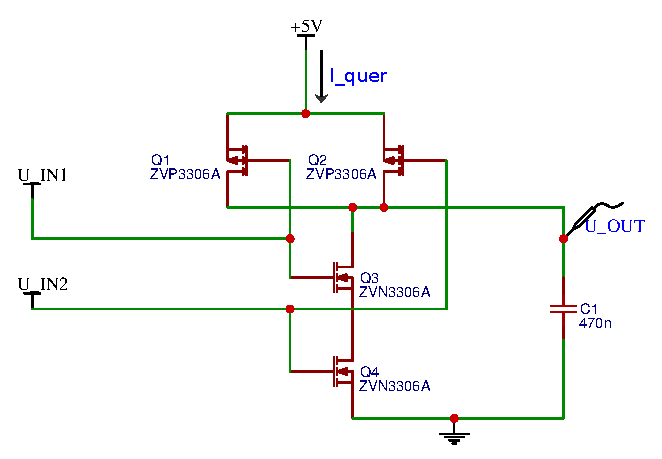
\includegraphics[width=\linewidth]{NAND.pdf}
        \caption{Aufbau des NAND-Gatters}
        \label{aufbauNAND}
    \end{minipage}% 
    \hfill
    \begin{minipage}[t]{0.45\linewidth}
        \centering
        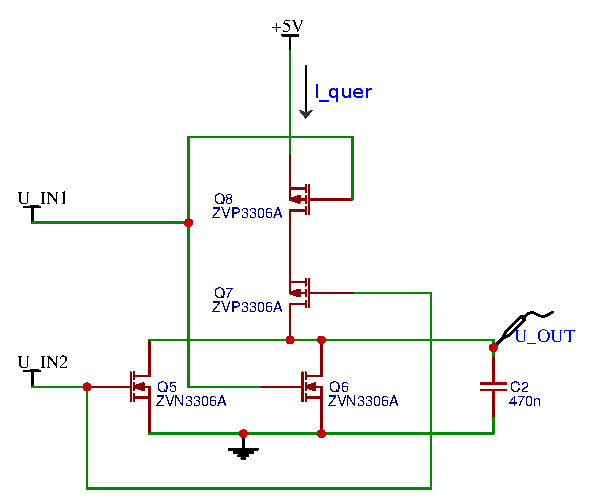
\includegraphics[width=\linewidth]{NOR.pdf}
        \caption{Aufbau des NOR-Gatters}
        \label{aufbauNOR}
    \end{minipage}
\end{figure}
\subsection*{Verwendete Bauteile}
\section*{Durchführung}. 
\section*{Messergebnisse}
\section*{Beobachtungen}
\section*{Auswertung}
\end{document}